% Qiskit Hackathon 2026 — Topic 5 — Team Garbage Collectors
% Build:  cd deck && pdflatex -interaction=nonstopmode slides.tex && pdflatex -interaction=nonstopmode slides.tex
% Every number carries its RESULTS.md row id. Do not edit numbers here without editing RESULTS.md.
\documentclass[aspectratio=169,11pt]{beamer}

\usetheme{default}
\usecolortheme{default}
\usepackage[T1]{fontenc}
\usepackage{lmodern}
\usepackage{amsmath,amssymb}
\usepackage{booktabs}
\usepackage{graphicx}
\usepackage{xcolor}

\definecolor{ink}{HTML}{0B0B0B}
\definecolor{blueA}{HTML}{2A78D6}
\definecolor{orangeA}{HTML}{EB6834}
\definecolor{aquaA}{HTML}{1BAF7A}
\definecolor{mutedA}{HTML}{898781}
\definecolor{bgA}{HTML}{FCFCFB}

\setbeamercolor{normal text}{fg=ink,bg=bgA}
\setbeamercolor{frametitle}{fg=ink,bg=bgA}
\setbeamercolor{structure}{fg=blueA}
\setbeamercolor{itemize item}{fg=blueA}
\setbeamercolor{itemize subitem}{fg=mutedA}
\setbeamertemplate{navigation symbols}{}
\setbeamertemplate{itemize item}{\textbullet}
\setbeamerfont{frametitle}{size=\large,series=\bfseries}
\setbeamertemplate{footline}{%
  \hspace{2ex}\tiny\color{mutedA}[R0xx] cites a numbered row in \texttt{RESULTS.md}\hfill%
  \tiny\color{mutedA}\insertframenumber/\inserttotalframenumber\hspace{2ex}\vspace{1ex}}

% every claim gets its source row
\newcommand{\src}[1]{{\tiny\color{mutedA}[#1]}}
\newcommand{\hl}[1]{{\color{blueA}\textbf{#1}}}
\newcommand{\mhl}[1]{{\color{blueA}\boldsymbol{#1}}}
\newcommand{\good}[1]{{\color{aquaA}\textbf{#1}}}
\newcommand{\bad}[1]{{\color{orangeA}\textbf{#1}}}

\title{\textbf{Garbage Collectors}}
\subtitle{Every Hadamard test throws away half its data. We recycle it.}
\author{\textbf{Team 8}\\ {\footnotesize TBD-NAME \and TBD-NAME \and TBD-NAME \and TBD-NAME \and TBD-NAME}}
\institute{\small Qiskit Hackathon 2026 --- Topic 5\\
\tiny after Faehrmann, Eisert \& Kueng, \emph{PRL} \textbf{135}, 150603 (2025)}
\date{\small 14 August 2026}

% section dividers: a "where are we" page before every section
\setbeamercolor{section in toc}{fg=ink}
\setbeamercolor{section in toc shaded}{fg=mutedA}
\setbeamerfont{section in toc}{size=\large,series=\bfseries}
\setbeamerfont{section in toc shaded}{size=\large,series=\mdseries}
\setbeamertemplate{section in toc shaded}[default][55]
\AtBeginSection[]{%
  \begin{frame}[plain]
    \vfill
    \centering
    \begin{minipage}{0.72\textwidth}
      \tableofcontents[currentsection, sectionstyle=show/shaded, hideallsubsections]
    \end{minipage}
    \vfill
  \end{frame}}

\begin{document}

\begin{frame}[plain]
  \titlepage
\end{frame}

\begin{frame}{Outline}
  \begin{minipage}{0.8\textwidth}
    \tableofcontents[hideallsubsections]
  \end{minipage}
  \vfill
  \begin{center}
  \small A tag like \src{R034} is not decoration --- it is a \hl{row number} in our
  public evidence ledger, \texttt{RESULTS.md}: 44 rows, one per reported number, each
  with the exact command that produced it. Full repo via the QR code on the last slide.
  \end{center}
\end{frame}

\section{The garbage state}

% ------------------------------------------------------------------ 1
\begin{frame}{Every Hadamard test throws away half its data}
  \begin{columns}[T]
    \begin{column}{0.54\textwidth}
      The standard Hadamard test measures \hl{one ancilla qubit}
      and \bad{discards the system register}.
      \medskip

      Measure that ``garbage'' in \emph{random bases} instead and it becomes a
      \hl{classical shadow} --- the same shots now also carry the system's observables.
      \medskip

      We implement this end to end, validate every estimate against exact references,
      \emph{quantify what it costs}, and characterise where it breaks.
    \end{column}
    \begin{column}{0.46\textwidth}
      \centering
      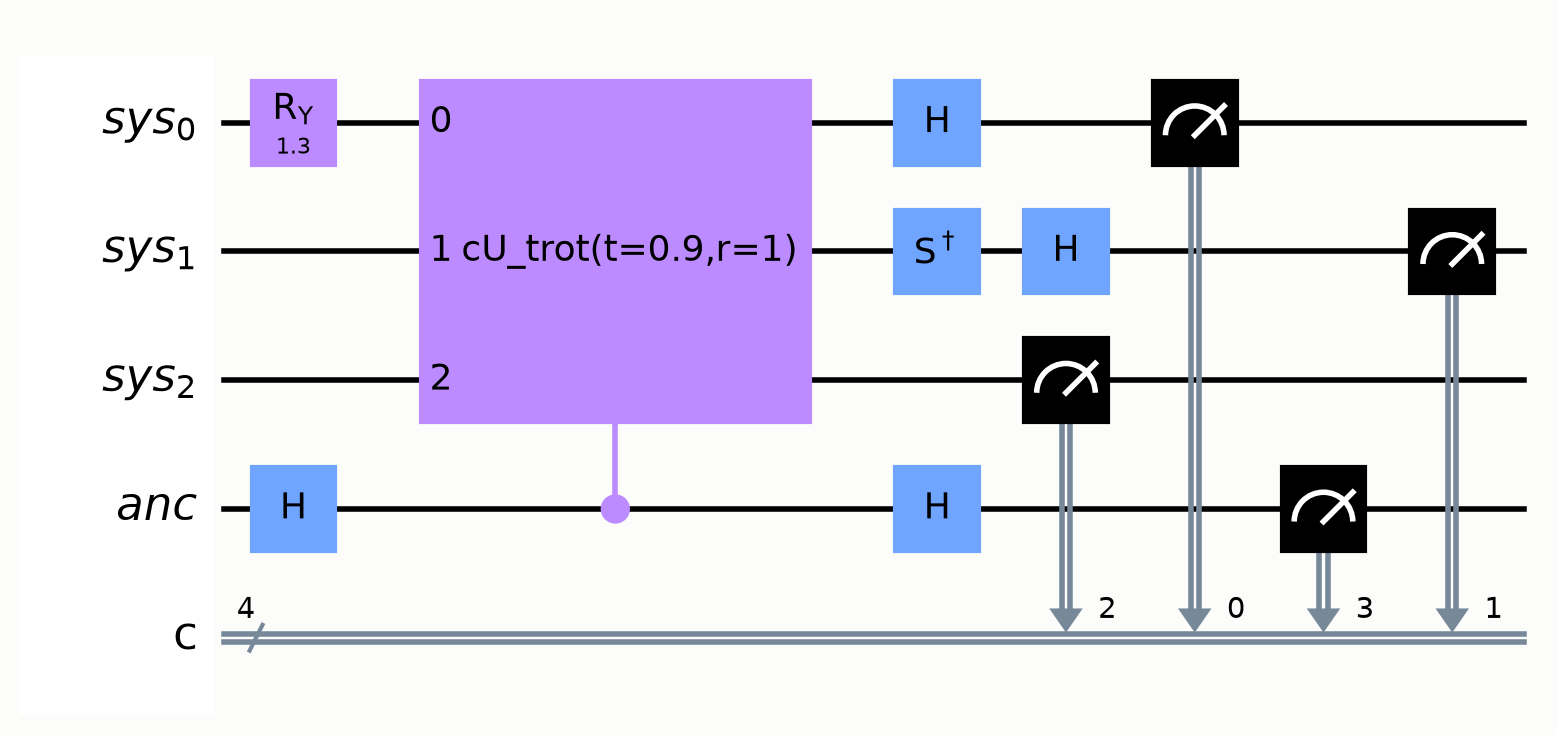
\includegraphics[width=\linewidth]{../figures/03_circuit_phi_0_real.png}\\
      \tiny\color{mutedA} 3 system qubits $+$ 1 ancilla
    \end{column}
  \end{columns}
\end{frame}

% ------------------------------------------------------------------ 1b  PAPER FIG 1
\begin{frame}{The protocol, in the authors' own picture}
  \vspace{-2mm}
  \begin{center}
    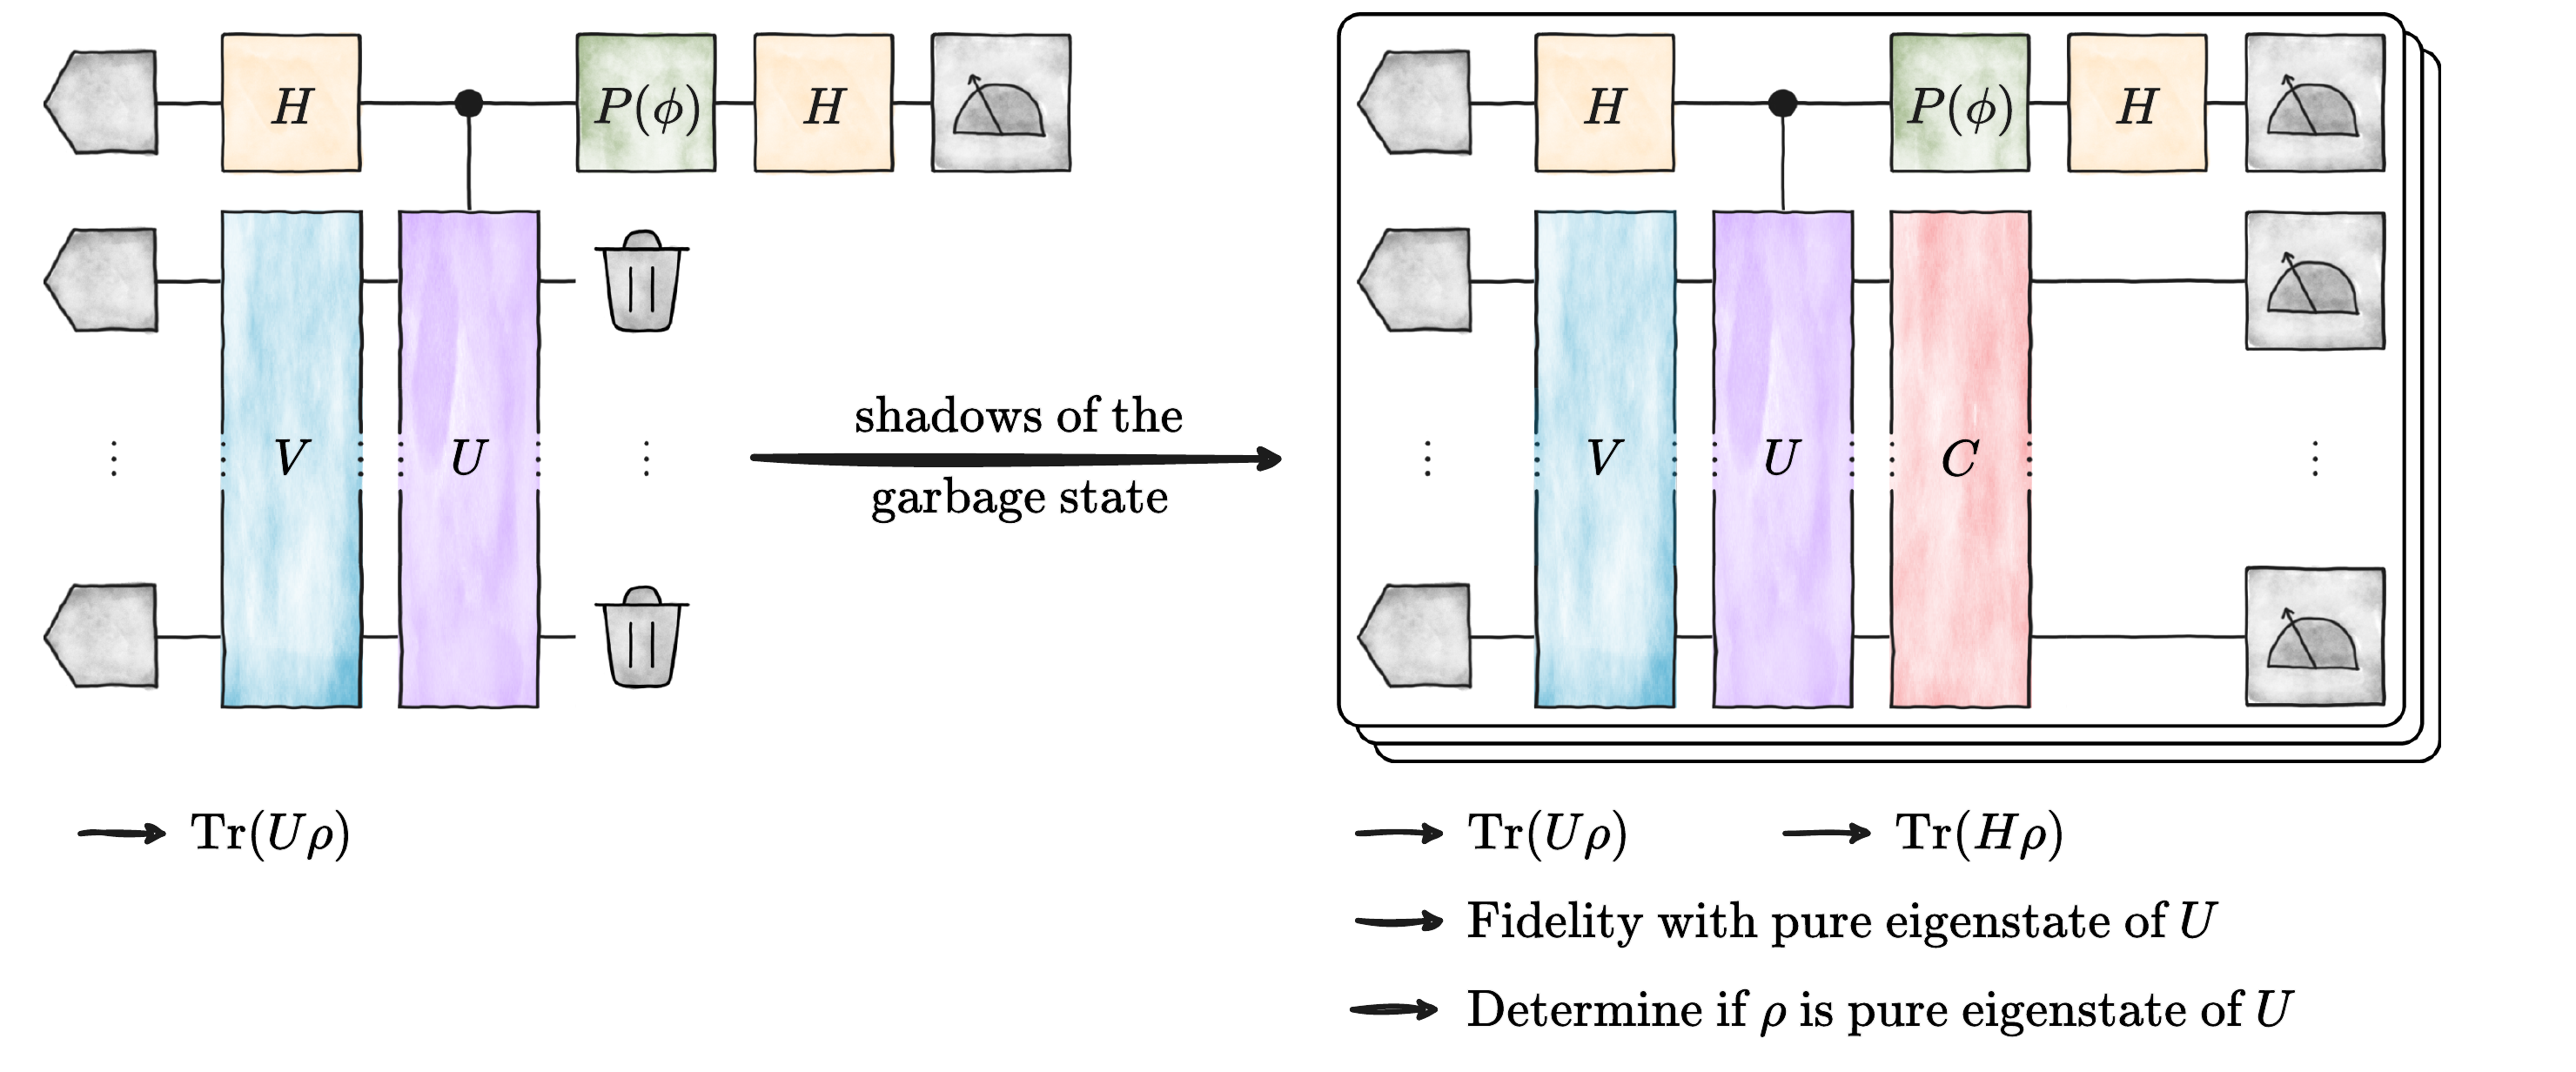
\includegraphics[width=0.88\linewidth]{fig_paper_fig1.png}
  \end{center}
  \vspace{-2mm}
  {\footnotesize
  \textbf{Left:} the standard test --- $V$ prepares, $c\text{-}U$ evolves, $P(\phi)$ picks
  the quadrature, and the system register goes \bad{in the bin}.
  \textbf{Right:} append a random Clifford $C$ and measure it instead:
  \hl{same circuit, same shots}, now also $\mathrm{Tr}(H\rho)$, fidelities and
  eigenstate tests.}
  \par\vspace{1mm}
  {\tiny\color{mutedA} Fig.~1 of Faehrmann, Eisert \& Kueng, \emph{PRL} \textbf{135},
  150603 (2025), reproduced under CC~BY~4.0. We use $\phi=-\pi/2$ for the imaginary
  quadrature, per the paper's body text (below its Eq.~2) and \texttt{CONVENTIONS \S5};
  the printed Fig.~1 caption reads $+\pi/2$.}
\end{frame}

% ------------------------------------------------------------------ 1c  SHADOWS
\begin{frame}{What a classical shadow actually is}
  \vspace{-2mm}
  \begin{center}
    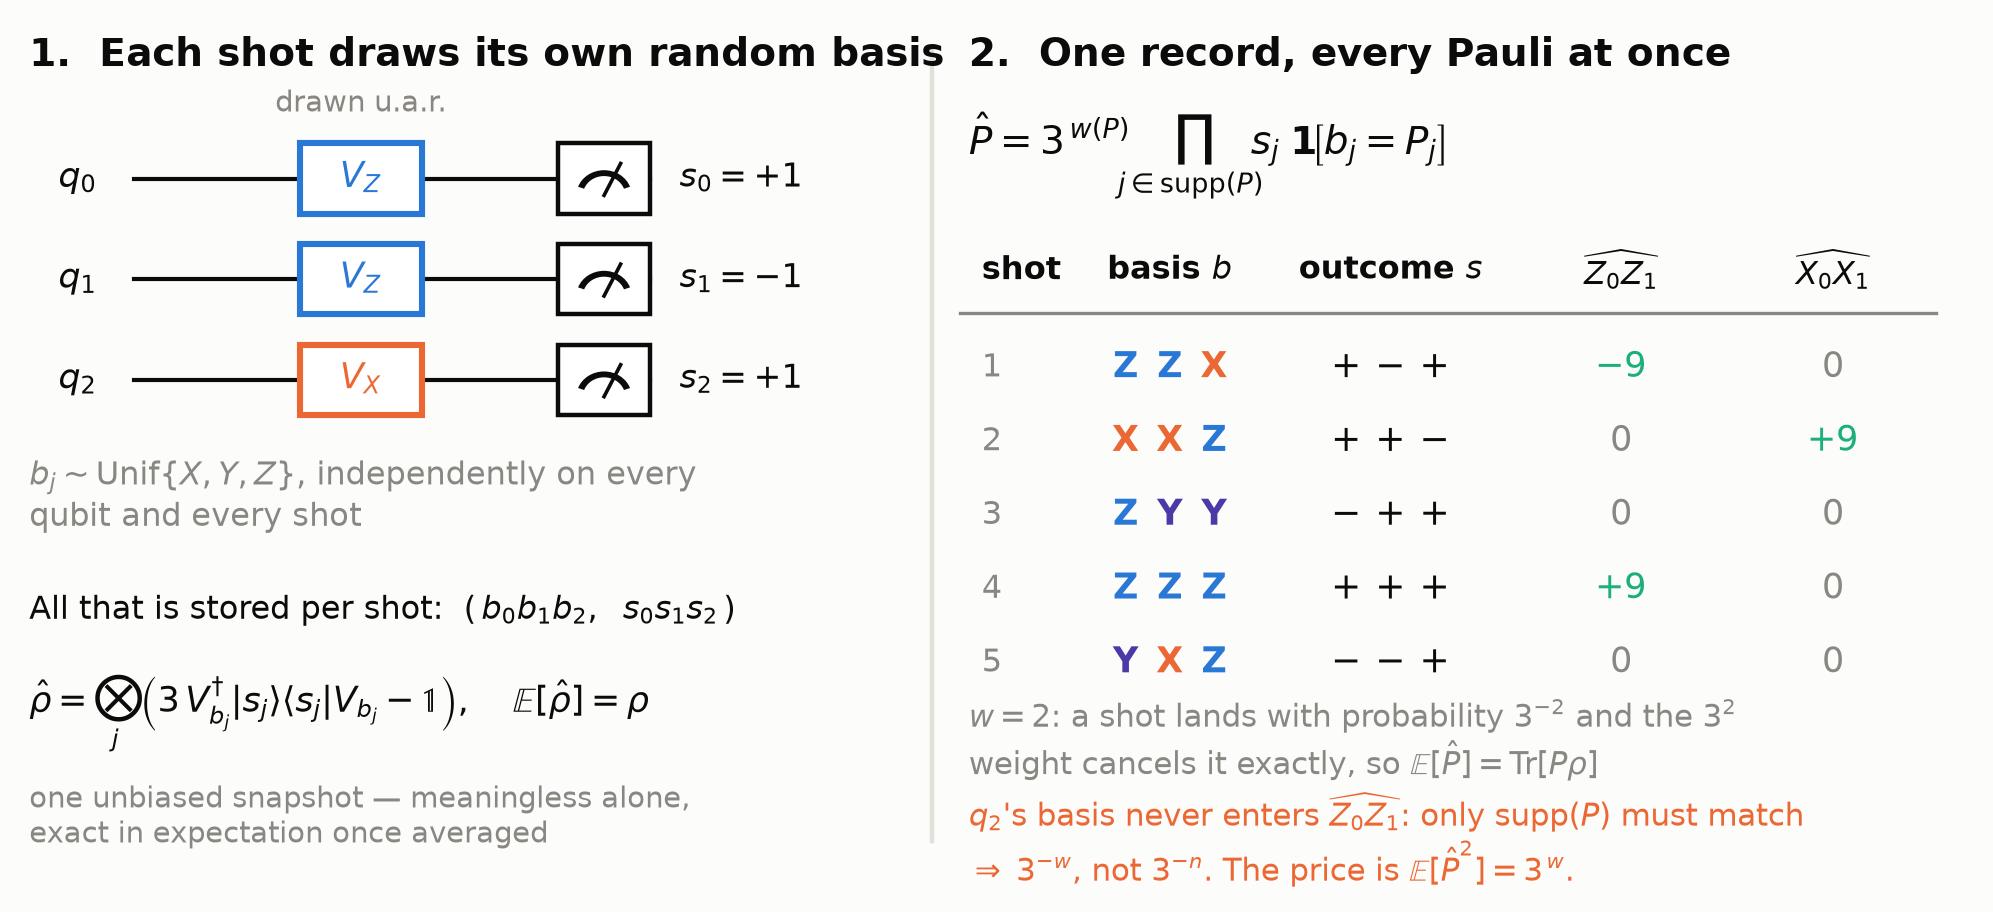
\includegraphics[width=0.90\linewidth]{fig_shadow.png}
  \end{center}
  \vspace{-2mm}
  {\footnotesize
  No new circuits --- only $\leq 2$ extra single-qubit gates per qubit. The randomisation is
  the whole trick: it is what makes \emph{one} record set an unbiased estimator for
  \hl{every} Pauli observable simultaneously, instead of one chosen in advance.
  \src{Hsin-Yuan Huang, Kueng \& Preskill, \emph{Nat.\ Phys.} \textbf{16}, 1050 (2020)}}
\end{frame}

% ------------------------------------------------------------------ 2
\begin{frame}{One circuit, one set of shots, seven physical quantities}
  The ancilla alone gives the interference signal:
  \[
    \langle Z_a\rangle_\phi \;=\; \mathrm{Re}\!\left[e^{i\phi}\,\mathrm{Tr}(U\rho)\right],
    \qquad \phi=0 \to \mathrm{Re}\,\chi,\quad \phi=-\tfrac{\pi}{2}\to \mathrm{Im}\,\chi
  \]
  Tracing out the ancilla leaves the \emph{unweighted} shadow target, and weighting each
  snapshot by the ancilla outcome $a=\pm1$ leaves the \emph{joint} one:
  \[
    \rho^{(I)}=\tfrac{1}{2}\bigl(\rho+U\rho U^{\dagger}\bigr),
    \qquad
    \mathbb{E}\bigl[a\,\hat P\bigr]=\mathrm{Re}\!\left[e^{i\phi}\mathrm{Tr}(P\,U\rho)\right]
  \]
  \begin{center}
  \small From \hl{one} record set: $\chi(t)$, $\chi_Q(t)$, $\chi_H(t)$, $\chi_{Z_0}(t)$,
  $\langle H\rangle$, $\langle Q\rangle$, $\langle Z_0\rangle$ \src{R009}
  \end{center}
  \begin{center}
  \textbf{3{,}456 circuits $\cdot$ 256{,}000 shots} --- one experiment, not seven.
  \end{center}
\end{frame}

% ------------------------------------------------------------------ 2b
\begin{frame}{The benchmark: three spins, nearest-neighbour coupling only}
  \vspace{-2mm}
  \begin{center}
    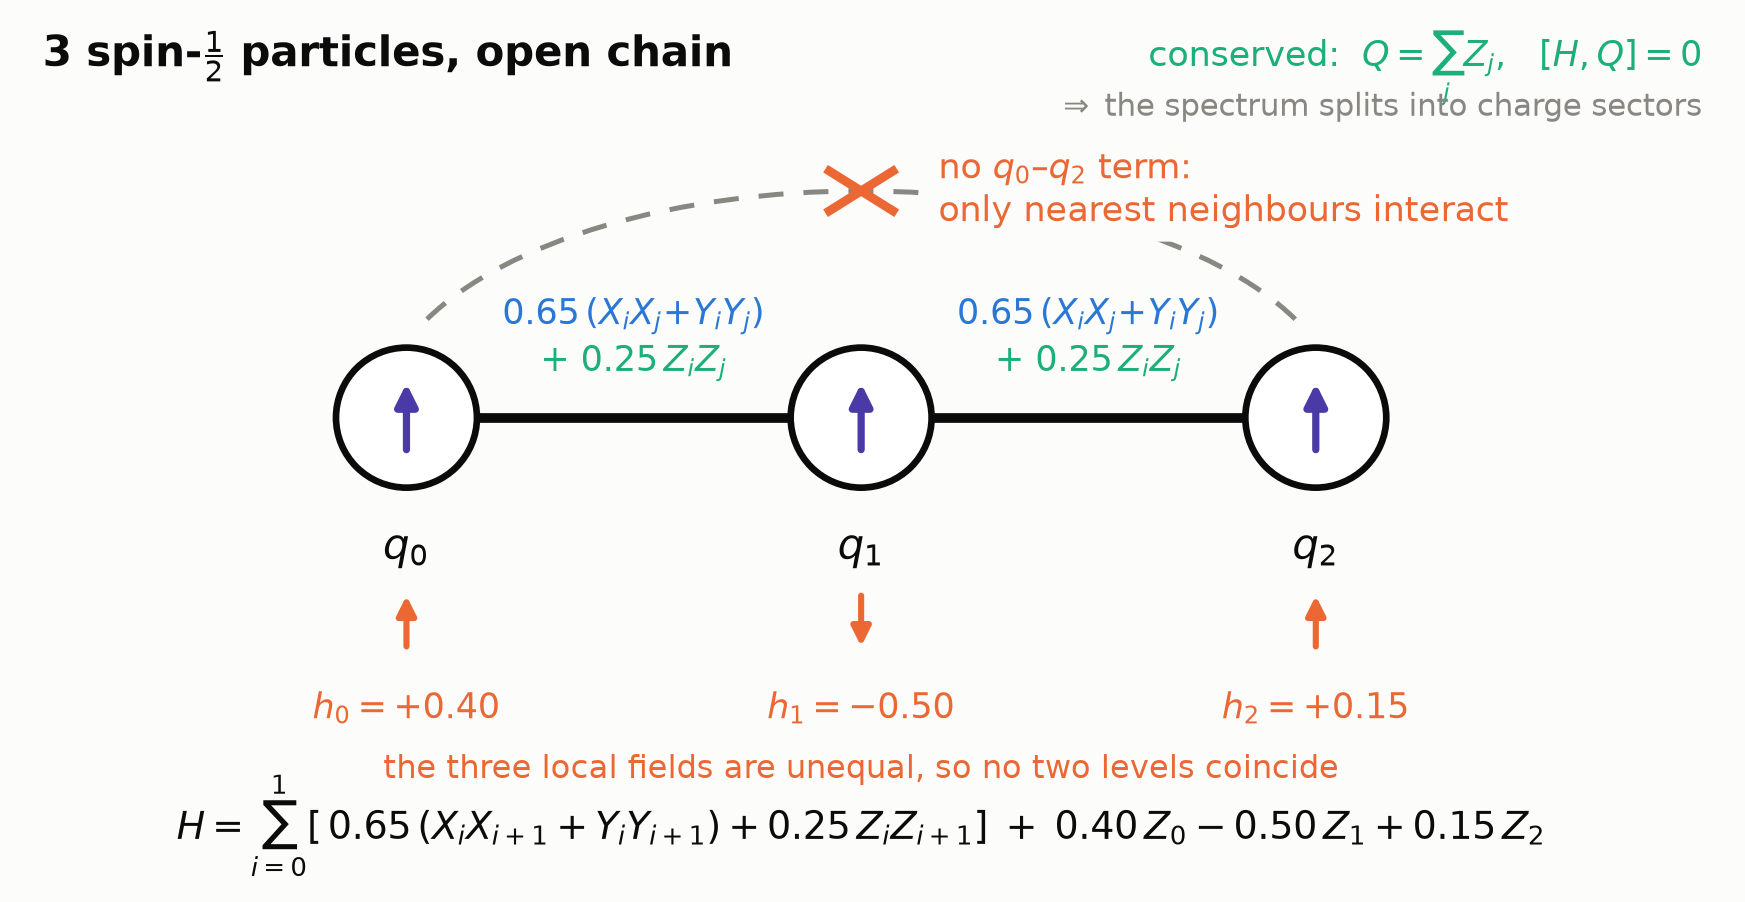
\includegraphics[width=0.86\linewidth]{fig_model.png}
  \end{center}
  \vspace{-2mm}
  {\footnotesize
  \textbf{Why this model.} Small enough to diagonalise exactly, so every estimate has a truth
  reference --- yet it still carries both features the protocol exploits: a
  \hl{conserved charge} and a \hl{non-degenerate spectrum}.
  \par\smallskip
  The initial state $R_y^{(q_0)}(1.3)\,|000\rangle$ reaches \hl{4 of the 8 levels}:
  $E\in\{-1.9152,\,-0.4810,\,+0.5500,\,+1.9463\}$ in sectors $q=+1,+1,+3,+1$.
  \src{R002, R012}}
\end{frame}

\section{Does it work?}

% ------------------------------------------------------------------ 3
\begin{frame}{Every estimator agrees with theory --- and the error bars are honest}
  \begin{columns}[T]
    \begin{column}{0.42\textwidth}
      \begin{itemize}
        \item \good{56/56 checkpoints pass}, zero hard failures, zero advisory warnings.
        \item $\chi(t)$ rms error \hl{0.0290} vs predicted sem \hl{0.0277}
              --- ratio \hl{1.05}, so the error bars neither over- nor under-state. \src{R010}
        \item Shot-noise slope \hl{$-0.463$} vs theory $-0.5$: unbiased,
              statistics-limited. \src{R010}
      \end{itemize}
      \medskip
      {\small The single-shot second moment is exactly $3^{w(P)}$, which predicts the
      measured error bars to \hl{within 2\%}. \src{R029}}
    \end{column}
    \begin{column}{0.58\textwidth}
      \centering
      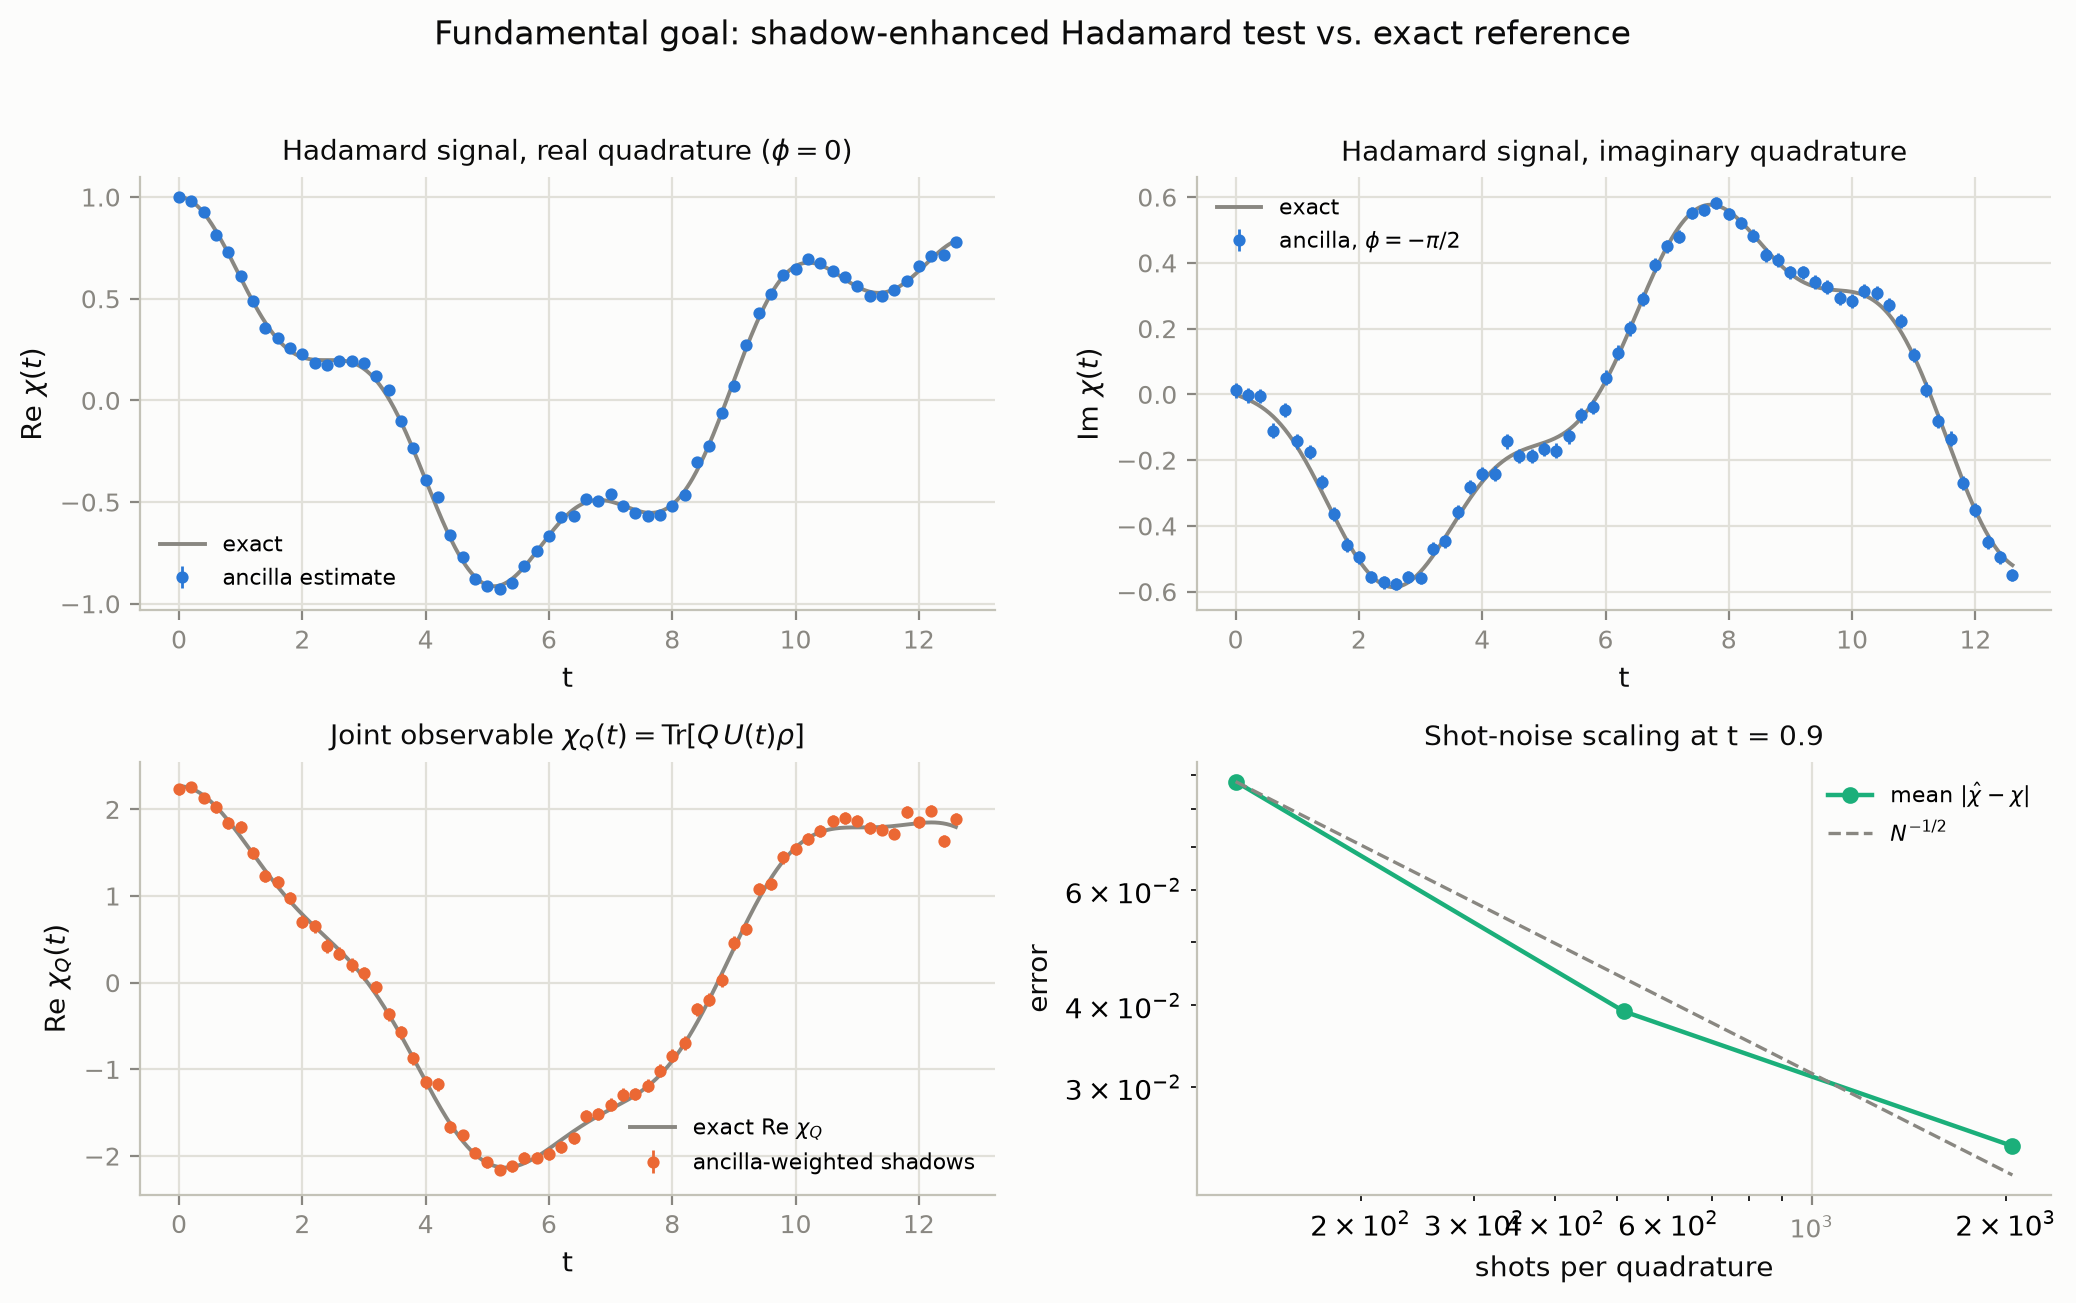
\includegraphics[width=\linewidth]{../figures/06_fundamental_validation.png}
    \end{column}
  \end{columns}
\end{frame}

% ------------------------------------------------------------------ 4
\begin{frame}{Conserved quantities come out flat --- from the very same shots}
  \begin{columns}[T]
    \begin{column}{0.57\textwidth}
      \centering
      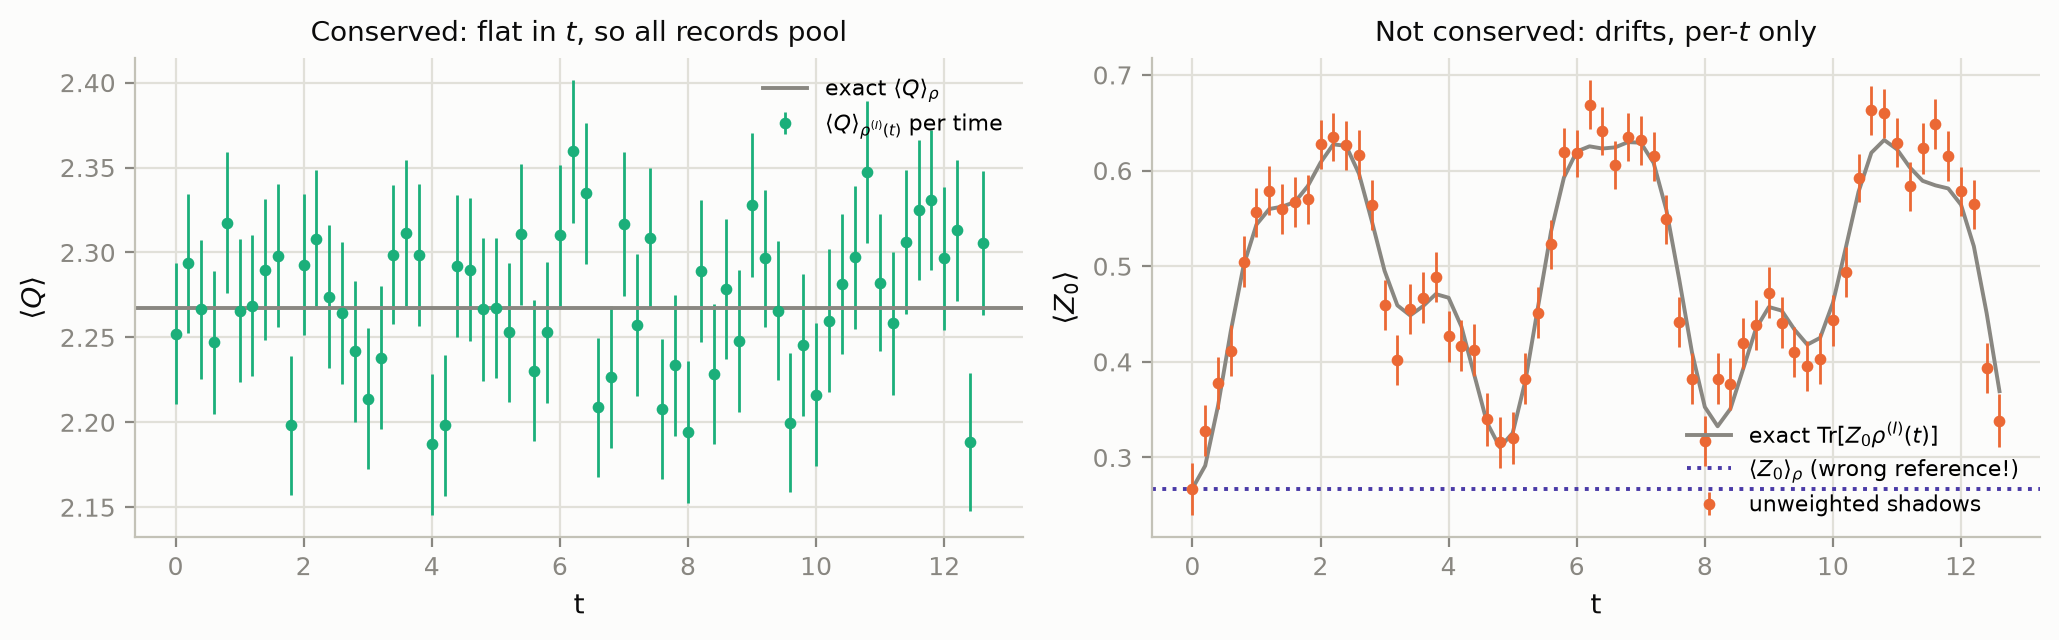
\includegraphics[width=\linewidth]{../figures/06_conservation.png}
    \end{column}
    \begin{column}{0.43\textwidth}
      \vspace{-2mm}
      \[ \langle H\rangle = \mhl{+0.0714 \pm 0.0082} \]
      \vspace{-6mm}
      \begin{center}\footnotesize exact $+0.0739$\end{center}
      \[ \langle Q\rangle = \mhl{+2.2708 \pm 0.0052} \]
      \vspace{-6mm}
      \begin{center}\footnotesize exact $+2.2675$\end{center}
      \smallskip
      \footnotesize
      Pooled over all 128 settings, extracted from the \emph{discarded} register of the
      $\chi(t)$ experiment. \src{R010}
      \medskip

      Per-time $\langle Q\rangle$ is flat within $5\sigma$ at every one of the 64 time
      points (max $2.2\sigma$). \src{R010}
      \medskip

      \textbf{No extra circuits} ($\leq 2$ extra 1-qubit gates per system qubit);
      the statistical cost is on slide~\ref{slide:cost}.
    \end{column}
  \end{columns}
\end{frame}

% ------------------------------------------------------------------ 5  MONEY PLOT
\begin{frame}{We recover the spectrum \emph{and} label each line by symmetry sector}
  \begin{columns}[T]
    \begin{column}{0.65\textwidth}
      \centering
      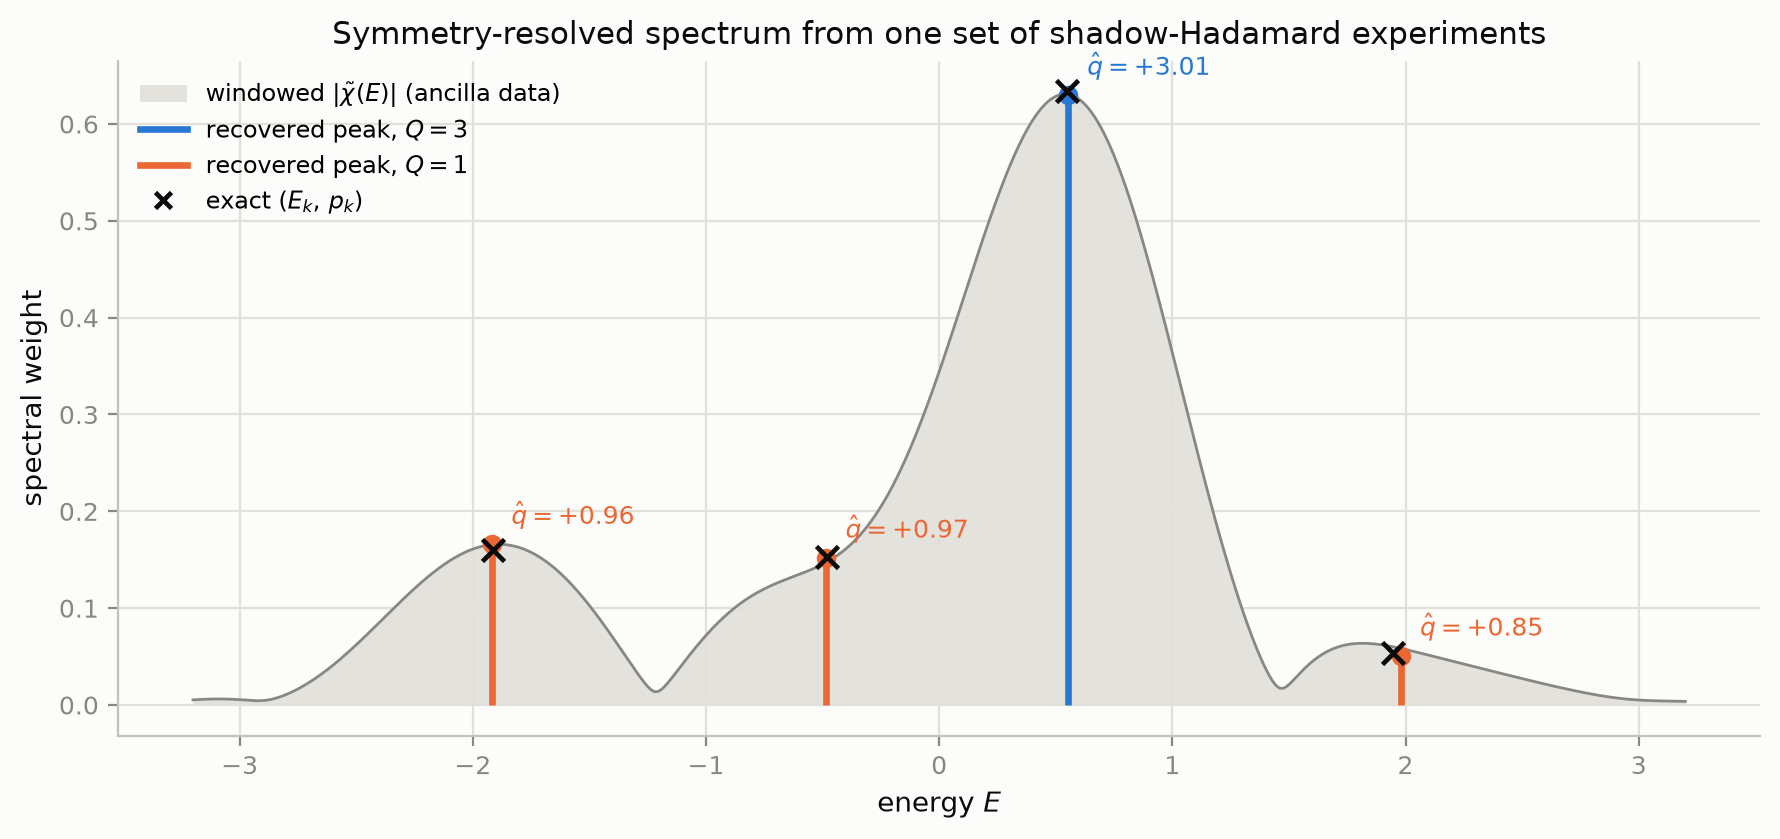
\includegraphics[width=\linewidth]{../figures/07_symmetry_resolved_spectrum.png}
    \end{column}
    \begin{column}{0.35\textwidth}
      \footnotesize
      All 4 populated levels recovered:\\
      max $|\Delta E| = $ \good{0.033}, max $|\Delta p| = $ \good{0.006},
      \good{every label correct}. \src{R012, R013}
      \medskip

      Reproducible: \good{12/12 independent seeds} got all four labels right. \src{R019}
      \medskip

      \textbf{The colour is the deliverable.} It is information the grey curve does not
      contain --- and it cost \emph{no additional circuits}.
      \medskip

      {\footnotesize\color{mutedA} The grey band is the plain windowed Fourier transform.
      A better estimator sharpens it; \emph{no} estimator can colour it.}
    \end{column}
  \end{columns}
\end{frame}

\section{What each choice buys}

% ------------------------------------------------------------------ 6
\begin{frame}{What each choice actually buys}
  \centering
  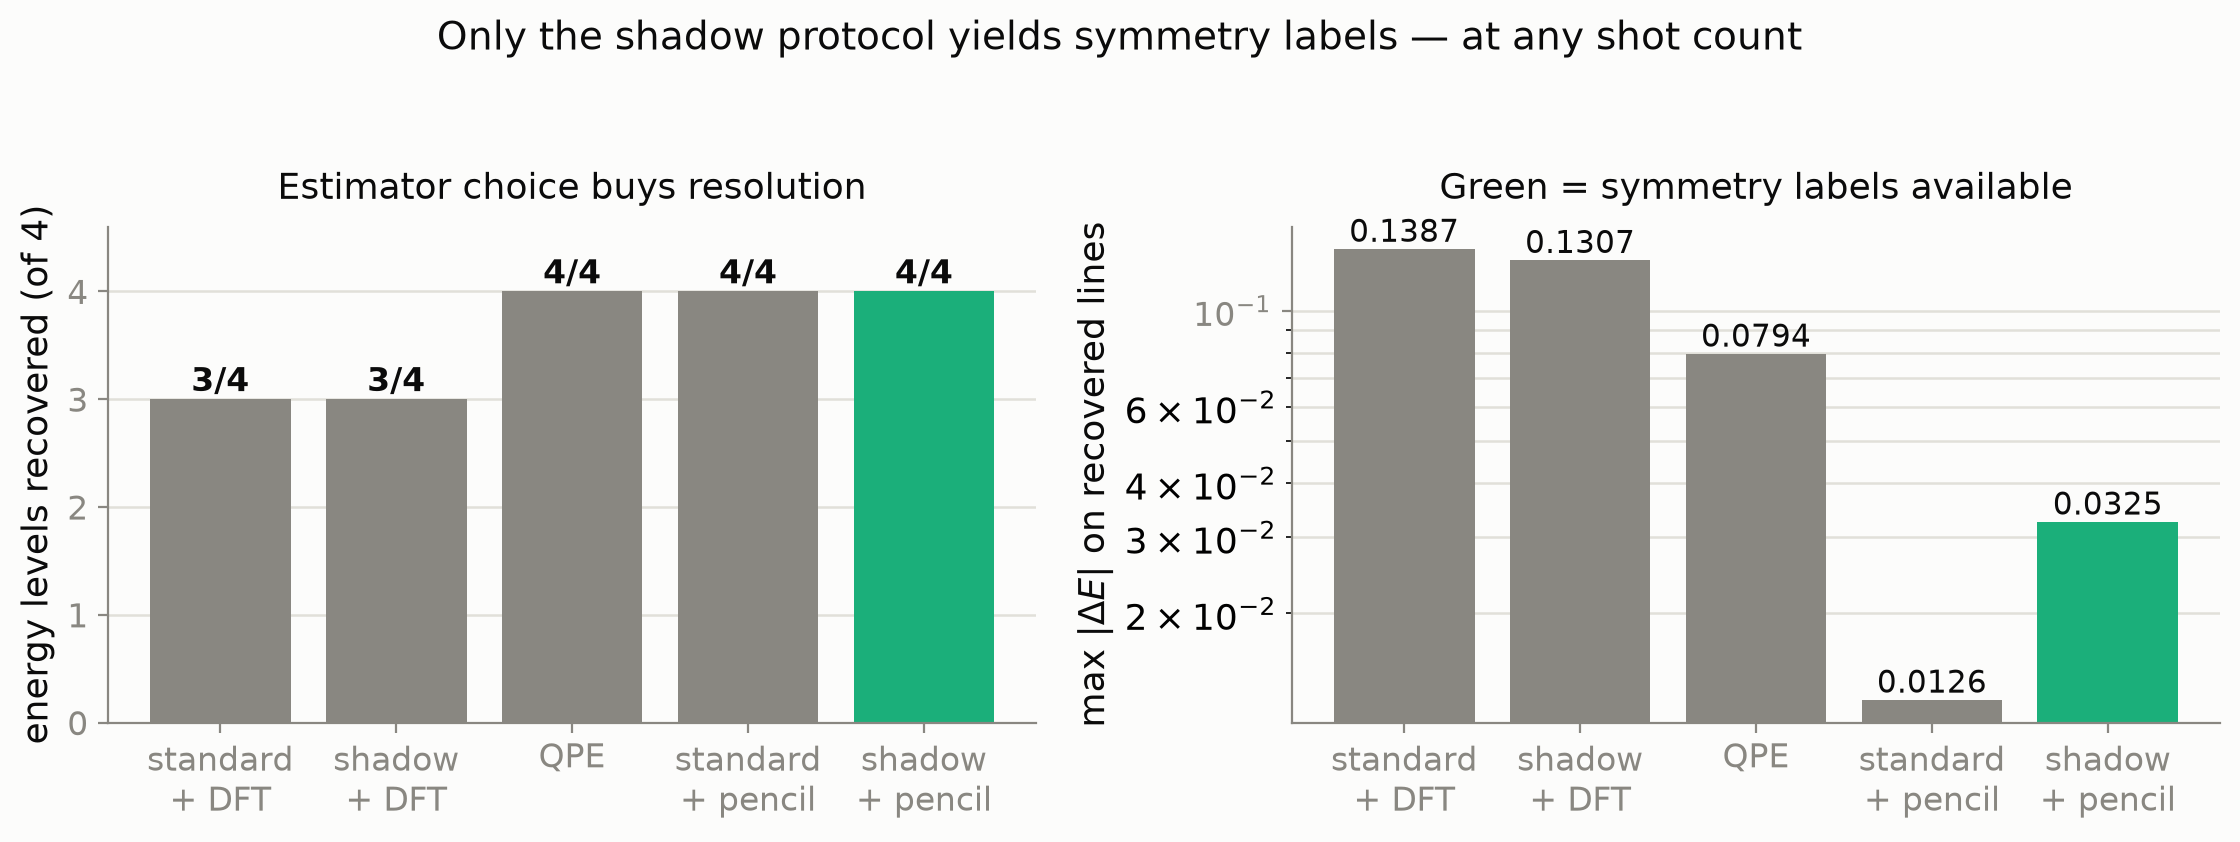
\includegraphics[width=0.99\linewidth]{fig_ablation.png}\\
  \smallskip
  \small
  \hl{Estimator} choice buys resolution ($3/4\to4/4$ lines).
  \hl{Protocol} choice buys the labels --- and nothing else can.
  \src{R011, R012, R021, R030}
\end{frame}

% ------------------------------------------------------------------ 6b  MOTIVATION
\begin{frame}{Do you even need shadows? Four ways to treat the garbage}
  \centering
  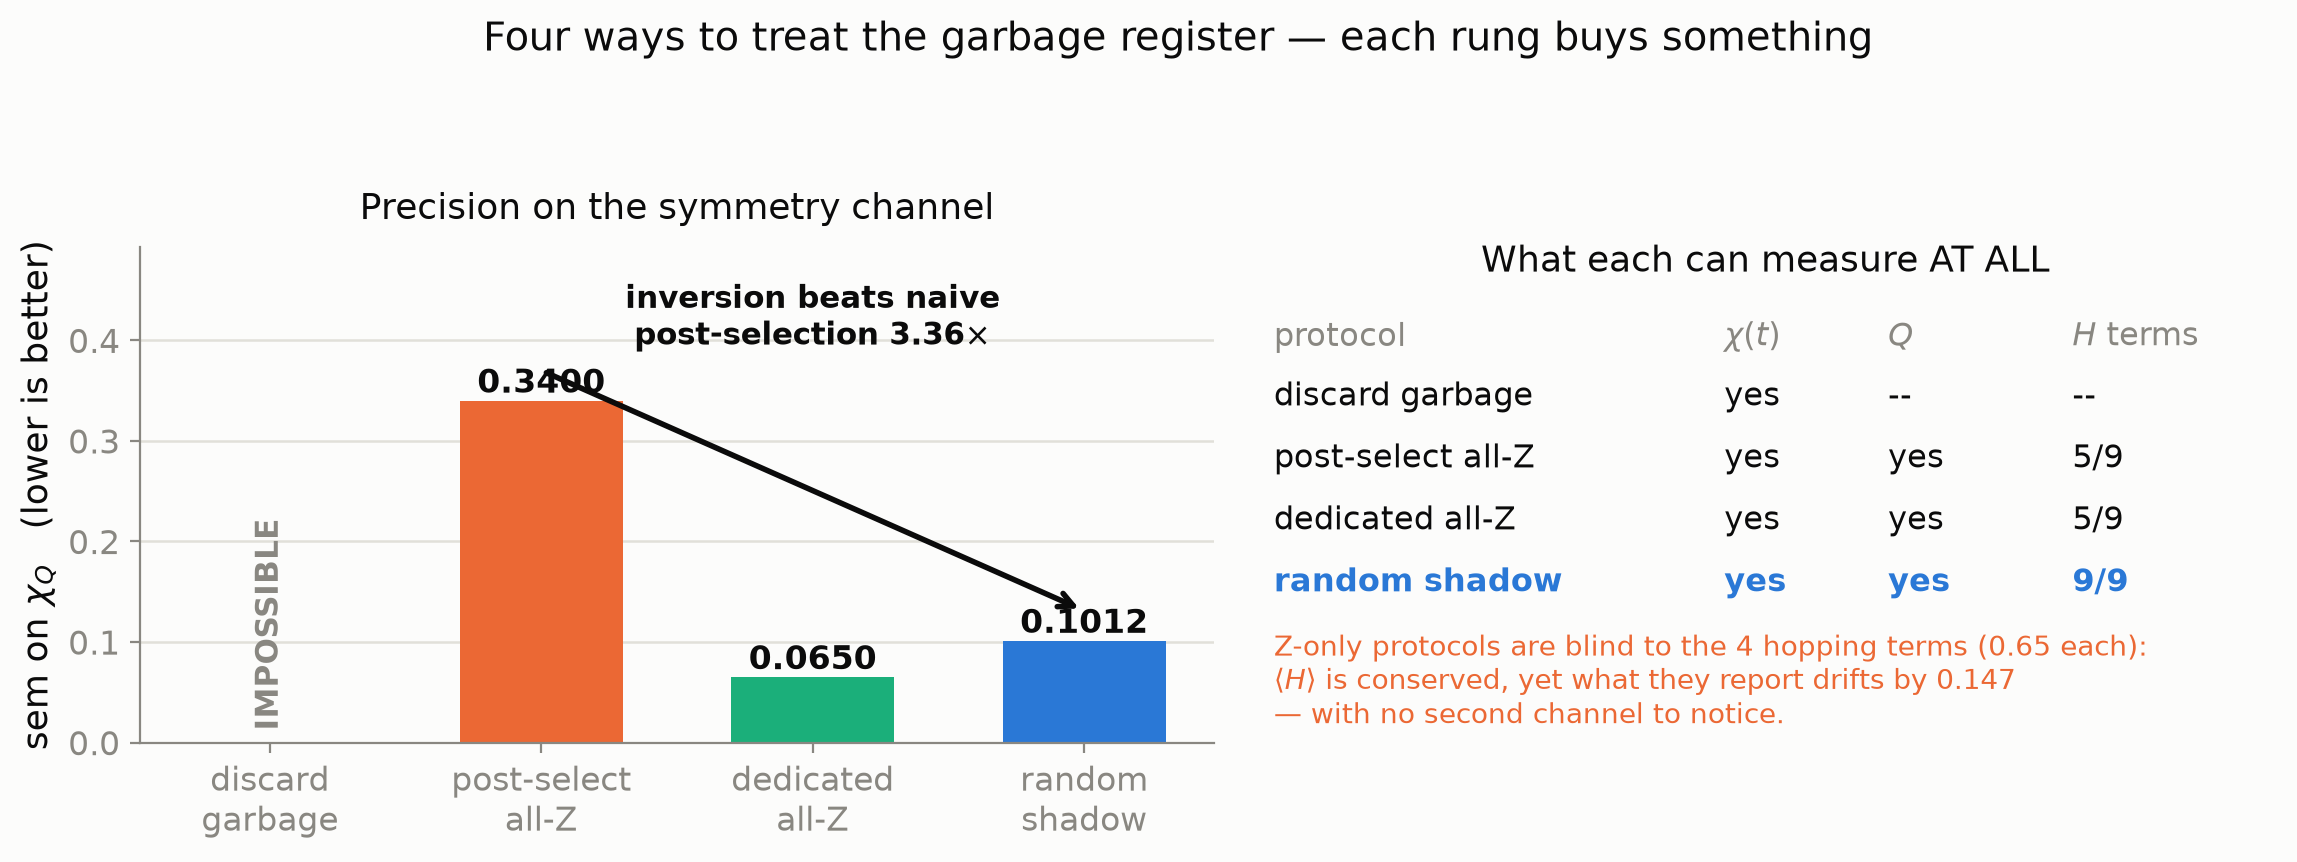
\includegraphics[width=\linewidth]{fig_escalation.png}\\
  \smallskip
  \small
  Each rung buys a capability the one below \emph{cannot have at any shot count}.
  \src{R039, R040}
\end{frame}

% ------------------------------------------------------------------ 6c
\begin{frame}{What the shadow inversion actually contributes}
  \small
  $Q=\sum_j Z_j$ is diagonal in the computational basis, so a \hl{dedicated Z readout beats
  our shadow estimator by 1.56$\times$} on the symmetry channel. We report that. \src{R039}
  \medskip

  But compare the shadow inversion against \emph{post-selecting the all-Z shots out of its
  own data}:
  \[
    \underbrace{\tfrac{1}{3}}_{\text{per \emph{term} } Z_j:\; b_j=Z}
    \qquad\text{versus}\qquad
    \underbrace{\tfrac{1}{3^{\,n}}}_{\text{\emph{all} qubits Z at once}}
    \;=\;3.7\%\ \text{of shots}
  \]
  \begin{center}
  \good{The inversion beats naive post-selection of the same data by 3.36$\times$}
  (sem $0.3400\to0.1012$) --- it recovers exactly the shots post-selection discards.
  \src{R040}
  \end{center}
  \medskip
  \centering
  \textbf{The case for shadows is not better symmetry resolution.}\\
  It is that the \emph{same} shots also give you $H$ --- which no Z-only protocol can see.
\end{frame}

% ------------------------------------------------------------------ 6d
\begin{frame}{Which protocol can rebuild which observable?}
  \scriptsize
  \begin{center}
  \begin{tabular}{llccc}
    \toprule
    \textbf{observable} & \textbf{what it measures physically}
      & \textbf{discard} & \textbf{post-select all-Z} & \textbf{shadow}\\
    & & {\tiny Hadamard $\to$ DFT} & {\tiny $\to$ matrix pencil} & {\tiny $\to$ matrix pencil}\\
    \midrule
    energies & the level structure of $H$
      & 3/4 lines & 4/4 & 4/4\\
    $Z_i$ & local magnetisation of spin $i$
      & \bad{---} & yes {\tiny(err 0.41 at 3.7\% yield)} & \good{yes} {\tiny(0.048)}\\
    $Z_iZ_j$ & neighbours \hl{aligned} vs \hl{anti-aligned}
      & \bad{---} & yes {\tiny(err 0.28)} & \good{yes} {\tiny(0.057)}\\
    $H$ & total energy
      & \bad{---} & \bad{biased} {\tiny(5/9 terms, 2.70)} & \good{yes} {\tiny(0.139)}\\
    $X_iX_j\!+\!Y_iY_j$ & \hl{hopping}: excitation exchanged between $i,j$
      & \bad{---} & \bad{impossible} {\tiny(0/2 terms)} & \good{yes} {\tiny(0.509)}\\
    \bottomrule
  \end{tabular}
  \end{center}
  \smallskip
  \small
  A Z-only protocol sees only what is \emph{diagonal}: it can say how the spins are
  \emph{oriented}, never how they \emph{move}. The hopping term is precisely the part of $H$
  that transports an excitation along the chain --- the part that makes the dynamics
  non-trivial --- and it converges to $\mathrm{Tr}[O_{Z\text{-diag}}U\rho]$, so more shots
  do not help.
  \par\smallskip
  \begin{center}
  \textbf{The shadow's exclusive capability is non-commuting observables.} \src{R041}
  \end{center}
\end{frame}

\section{Real hardware, and the price}

% ------------------------------------------------------------------ 7
\begin{frame}{It survives on real hardware once the circuit is shallow enough}
  \begin{columns}[T]
    \begin{column}{0.61\textwidth}
      \centering
      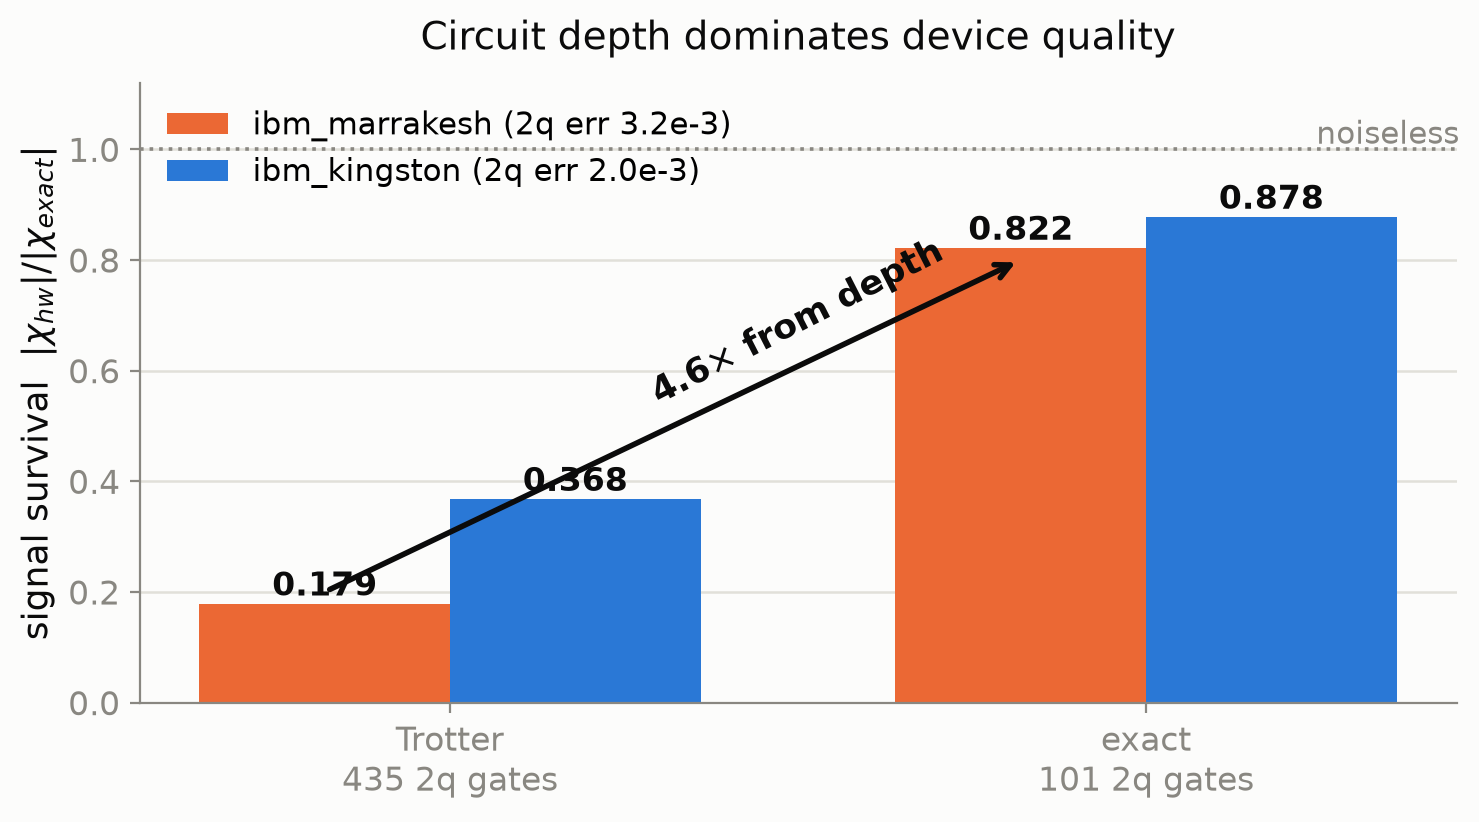
\includegraphics[width=\linewidth]{fig_hardware_grid.png}
    \end{column}
    \begin{column}{0.39\textwidth}
      \footnotesize
      Complete $2\times2$ grid. Depth dominates (\hl{2.4--4.6$\times$}) over device choice
      (1.1--2.1$\times$). \src{R008, R018}
      \medskip

      With a \emph{full random-basis ensemble} on hardware:
      $\chi$ survival \good{0.962}, and a valid
      $\langle Q\rangle$ at \good{0.957} --- the core claim, on a real QPU. \src{R023}
      \medskip

      {\footnotesize\color{orangeA}\textbf{Caveat, stated plainly:} one run per
      configuration. An independent run of an identical circuit 30 minutes later differed
      by $>2\times$. Hardware varies; we report that. \src{R026, R031}
      \par\smallskip
      \textbf{And a deeper test failed, on both devices:} at $n{=}6$ a 576-gate AQC
      circuit returned \bad{0.026} / \bad{0.033} against pre-registered $0.315$ / $0.401$
      --- the compilation advantage does \emph{not} reach hardware yet. \src{R054}}
    \end{column}
  \end{columns}
\end{frame}

% ------------------------------------------------------------------ 8
\begin{frame}{The honest cost: 13 experiments replaced for a 1.07$\times$ variance premium}
  \label{slide:cost}
  The per-shot Pauli estimator and its exact second moment:
  \[
    \hat P \;=\; 3^{\,w(P)}\prod_{j\in \mathrm{supp}(P)} s_j\;
    \mathbf{1}\!\left[b_j = P_j\right],
    \qquad
    \mathbb{E}\bigl[\hat P^{2}\bigr] \;=\; 3^{\,w(P)}
  \]
  \begin{columns}[T]
    \begin{column}{0.5\textwidth}
      \small
      Conventional route: \hl{13 dedicated} modified Hadamard tests
      ($Q\!=\!3$, $H\!=\!9$, $Z_0\!=\!1$ Pauli terms).
      \medskip

      Shadow route: \hl{0 extra circuits}
      ($\leq2$ extra 1q gates per qubit).
    \end{column}
    \begin{column}{0.5\textwidth}
      \small
      Price paid instead --- measured, not asserted:
      \[
        \frac{\mathrm{sem}_{\text{shadow}}}{\mathrm{sem}_{\text{dedicated}}}
        = \frac{0.1012}{0.0949} = \mhl{1.07\times}
      \]
      on $\chi_Q$ specifically. \src{R021}
    \end{column}
  \end{columns}
  \medskip
  \centering\small
  The $3^{w}$ model predicts the observed error bars to \good{within 2\%}. \src{R029}
\end{frame}

\section{Reproduce it, and where it breaks}

% ------------------------------------------------------------------ 9
\begin{frame}{Reproduce it in under five minutes}
  \begin{columns}[T]
    \begin{column}{0.55\textwidth}
      \small
      \begin{itemize}
        \item \hl{44 sourced results rows} --- every number maps to the command that
              produced it (\texttt{EVIDENCE.md}).
        \item Quickstart reproduces our headline \emph{table} from saved data; the money
              plot ships pre-rendered.
        \item \texttt{hardware\_run.py} reproduces our hardware arm in 3 commands.
        \item \texttt{BUGLOG.md} --- including the numbers we got wrong and retracted.
      \end{itemize}
    \end{column}
    \begin{column}{0.45\textwidth}
      \centering
      
\includegraphics[width=0.62\linewidth]{qr_slides.png}\\
      {\tiny\color{mutedA} \texttt{github.com/mnsh0409/Qiskit-Hackathon-2026}}
    \end{column}
  \end{columns}
  \vfill
  {\footnotesize\color{mutedA} First open implementation of PRL \textbf{135}, 150603.
  Prior-art search 2026-08-13; scope and limits recorded in
  \texttt{deck/PRIOR\_ART\_SEARCH.md}.}
\end{frame}

% ------------------------------------------------------------------ 10
\begin{frame}{What we could not do, and where it breaks}
  \small
  \begin{itemize}
    \item The windowed DFT \bad{never} resolves the 1.031-spaced pair at \emph{any}
          $T_{\max}$ we tested; the matrix pencil resolves it from $T_{\max}\geq7.0$.
          A method limit, not a shot-count limit. \src{R011, R022}
    \item Exact-synthesis shallowness is an \bad{$n{=}3$ artefact} --- the advantage falls
          $3.41\times\!\to\!1.16\times$ from $n{=}3$ to $n{=}4$ and is \emph{expected} to
          invert beyond (measured at $n{=}3,4$ only). Not a scalable recipe. \src{R025}
    \item One noise study came out \bad{confounded}; we exclude it rather than report it.
          \src{R017}
    \item Hardware supports \emph{robustness claims only} --- never a headline number.
          All Part A/B results are simulator.
  \end{itemize}
  \vfill
  \centering
  \textbf{We make no claim of outperforming classical computation.}\\
  {\small The system is 3 qubits; a laptop diagonalises it instantly. It is small
  \emph{on purpose}, so every estimate can be graded against an exact answer.}
\end{frame}

% ------------------------------------------------------------------ 11
\begin{frame}{Team 8 --- Garbage Collectors}
  \begin{itemize}
    \item \textbf{TBD-NAME} --- TBD-CONTRIBUTION (script block M1)
    \item \textbf{TBD-NAME} --- TBD-CONTRIBUTION (M2)
    \item \textbf{TBD-NAME} --- TBD-CONTRIBUTION (M3)
    \item \textbf{TBD-NAME} --- TBD-CONTRIBUTION (M4)
    \item \textbf{TBD-NAME} --- TBD-CONTRIBUTION (M5)
  \end{itemize}
  \vfill
  \centering
  \Large\textbf{Team 8 --- Garbage Collectors}\\
  \normalsize Thank you --- questions welcome.
\end{frame}

\begin{frame}{References}
  \footnotesize
  \textbf{Papers}
  \begin{itemize}\itemsep 2pt
    \item[{[1]}] P.~K. Faehrmann, J. Eisert, R. Kueng, Phys.\ Rev.\ Lett.\ \textbf{135},
      150603 (2025); arXiv:2505.15913 --- the protocol; Fig.~1 reproduced on slide
      ``The protocol, in the authors' own picture'' under CC~BY~4.0.
    \item[{[2]}] H.-Y. Huang, R. Kueng, J. Preskill, Nat.\ Phys.\ \textbf{16}, 1050 (2020)
      --- classical shadows.
    \item[{[3]}] S. Khatri, R. LaRose, A. Poremba, L. Cincio, A.~T. Sornborger, P.~J. Coles,
      Quantum \textbf{3}, 140 (2019) --- Hilbert--Schmidt test.
    \item[{[4]}] Goh \& Koczor, arXiv:2407.03414 --- fermionic density of states
      (backup slide ``future work'').
  \end{itemize}
  \smallskip
  \textbf{Software} \quad Qiskit 2.5.1; qiskit-ibm-runtime 0.49;
  \texttt{qiskit-addon-aqc-tensor} 0.3.1; quimb [J. Gray, JOSS \textbf{3}(29), 819 (2018)]
  $+$ JAX. \quad \textbf{Benchmark:} the Topic-5 participant notebook (XXZ model,
  Tracks A--E). All other figures are our own, script-generated.
\end{frame}

% ================================================================== BACKUP
\appendix
\begin{frame}[plain]
  \centering\Large\textbf{Backup slides}
\end{frame}

\begin{frame}{Backup --- the standard and shadow protocols give \emph{identical} $\chi$}
  \small
  Measured, not assumed: a genuine textbook Hadamard test over the full 64-point grid at
  identical budget gives
  \[
    \text{rms}_{\text{std}} = 0.0265,\quad \text{rms}_{\text{shadow}} = 0.0290,
    \qquad \text{mean sem } 0.0277 \text{ vs } 0.0277
  \]
  with $|\chi_{\text{std}}-\chi_{\text{shadow}}|/\text{combined sem}$: max $2.10\sigma$,
  mean $0.88\sigma$ --- statistically the \hl{same random variable}. \src{R021}
  \medskip

  So measuring the garbage register costs the ancilla signal \emph{nothing}, and the two
  axes factorise cleanly: estimator $\to$ resolution, protocol $\to$ labels.
\end{frame}

\begin{frame}{Backup --- a self-validating decoherence witness}
  For a pure input state, exactly:
  \[
    \mathrm{Tr}\!\left[(\rho^{(I)})^{2}\right] \;=\; \tfrac{1}{2}\left(1+|\chi(t)|^{2}\right)
  \]
  \small
  Left side from the \hl{system register alone} (shadow snapshot pairs); right side from the
  \hl{ancilla alone}. Two independent channels of the same experiment, so their gap
  certifies decoherence with \good{no exact diagonalisation and no classical simulation} ---
  it survives to sizes where nothing can be verified.
  \medskip

  \centering
  \begin{tabular}{lr}
    \toprule
    ideal simulator & $-0.1\sigma$ \quad(correct null)\\
    noisy sim, $1\times$ & $-7.6\sigma$ \quad(fires)\\
    noisy sim, $5\times$ & $-17.2\sigma$ \quad(dose-response)\\
    real hardware (cleanest run) & $-1.4\sigma$ \quad(correct null)\\
    \bottomrule
  \end{tabular}
  \\[0.5em] \src{R033}
\end{frame}

\begin{frame}{Backup --- future work, already prototyped: density of states}
  The DOS is the Fourier transform of the \emph{trace} of the propagator:
  \[
    G(t) \;=\; \frac{1}{\sqrt{2\pi}}\,\mathrm{Tr}\!\left[e^{-i\hat H t}\right]
    \qquad\text{\scriptsize (Goh \& Koczor, arXiv:2407.03414v2, Eq.~7)}
  \]
  \small
  Our $\chi(t)=\mathrm{Tr}[U(t)\rho]$. Set $\rho = \mathbb{1}/2^n$ and \hl{the same
  experiment becomes a DOS estimator} --- one line changed, analysis chain untouched.
  \medskip

  Prototyped: peak weights correctly become \emph{degeneracies}
  (isolated levels $0.11$--$0.13$ vs predicted $1/8$; a 3-fold merged peak
  $0.354$ vs predicted $3/8$). \src{R038}
  \medskip

  \textbf{Where we could improve on that paper:} it obtains fixed-particle-number DOS with
  \emph{one experiment per sector}. Our shadow channel measures $\langle Q^k\rangle$ from
  the \emph{same} shots, so the charge moments at each peak recover \hl{all sectors from a
  single run}. Feasibility checked: $Q^2,Q^3$ are 4 Pauli terms each; moment inversion
  condition number 31.
\end{frame}

\begin{frame}{Backup --- where SKQD helps, and why not here}
  \vspace{-2mm}
  \begin{center}
    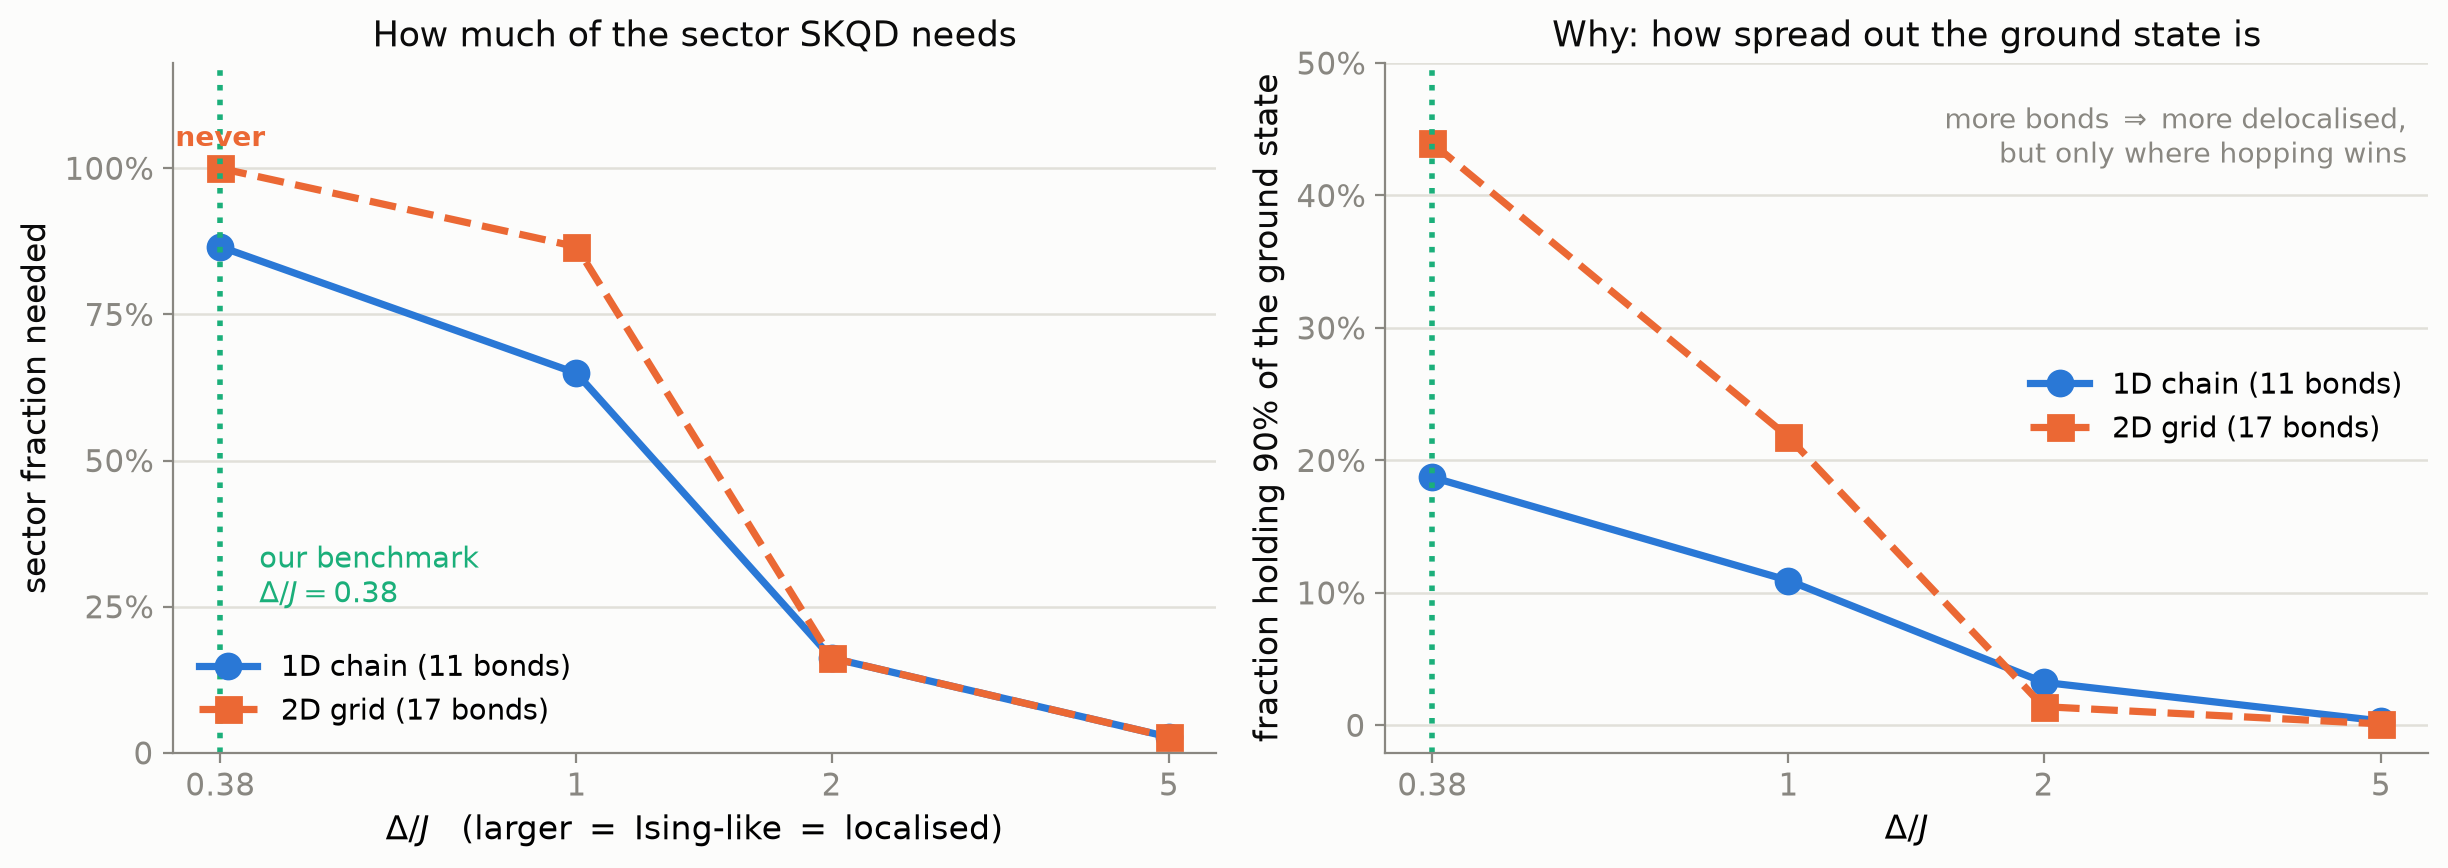
\includegraphics[width=0.72\linewidth]{fig_skqd_boundary.png}
  \end{center}
  \vspace{-3mm}
  {\scriptsize
  SKQD spans a subspace instead of enumerating one, and its advantage is governed by
  \hl{how localised the ground state is}. On our benchmark ($\Delta/J{=}0.38$) it needs
  \bad{86.6\%} of the charge sector; at $\Delta/J{=}5$ only \good{2.7\%}. \src{R047}
  \ In \textbf{2D} (11 bonds $\to$ 17, same sector) it is \bad{worse where hopping dominates}
  and \good{identical once localised}. \src{R048}
  \par\smallskip
  \textbf{Real physics, or our toy model?} Repeated on \hl{2D Fermi--Hubbard} (12 qubits,
  half filling), knob $U/t$: same boundary --- \good{12.5\%} of the sector at $U/t{=}16$
  (Mott), \bad{never} for $U/t\leq4$ (metallic). That is why SQD succeeds in chemistry and
  not here. \src{R050}
  \par\smallskip
  \textbf{And the part that DID work, on a real QPU:} \hl{symmetry-based configuration
  recovery} on our kingston shots removed \emph{exactly} the artefact noise introduced ---
  66/4{,}000 charge-violating shots leaked one \bad{spurious eigenvalue} ($+0.35$) into the
  subspace; recovery: dim $4\to3$, spurious \bad{1}$\,\to\,$\good{0}, with no reference
  state and no simulation. \src{R037}}
\end{frame}

\begin{frame}{Backup --- two bugs we caught, and how}
  \small
  \textbf{B04 --- a fixed-basis shadow estimator silently returns a \emph{different}
  observable.} The estimator is unbiased only for i.i.d.-uniform bases; with one fixed basis
  the indicator is deterministic and non-matching terms contribute structurally zero. We
  reported a hardware $\langle Q\rangle$ this way and blamed noise. On a \emph{noiseless}
  simulator the same code is \bad{65$\sigma$ off} --- so it was never noise. Retracted;
  \texttt{hardware\_run.py} now refuses to print system observables without
  \texttt{-{}-shadow}.
  \medskip

  \textbf{B06 --- an error bar computed over the wrong units.} Purity is a U-statistic over
  \emph{pairs} of snapshots; we used $\mathrm{std}/\sqrt{n_{\text{pairs}}}$, but pairs share
  shots, so the effective sample size is the number of \emph{shots}. That faked a
  $2.2\sigma$ signal. \good{Only the ideal-simulator control leg exposed it} --- the
  hardware number alone looked fine.
  \medskip

  \centering\emph{A witness validated only where the truth is unknown cannot be trusted.}
\end{frame}

\end{document}
